%!TEX root = ../../main.tex


\begin{figure}[!htb]
\centering
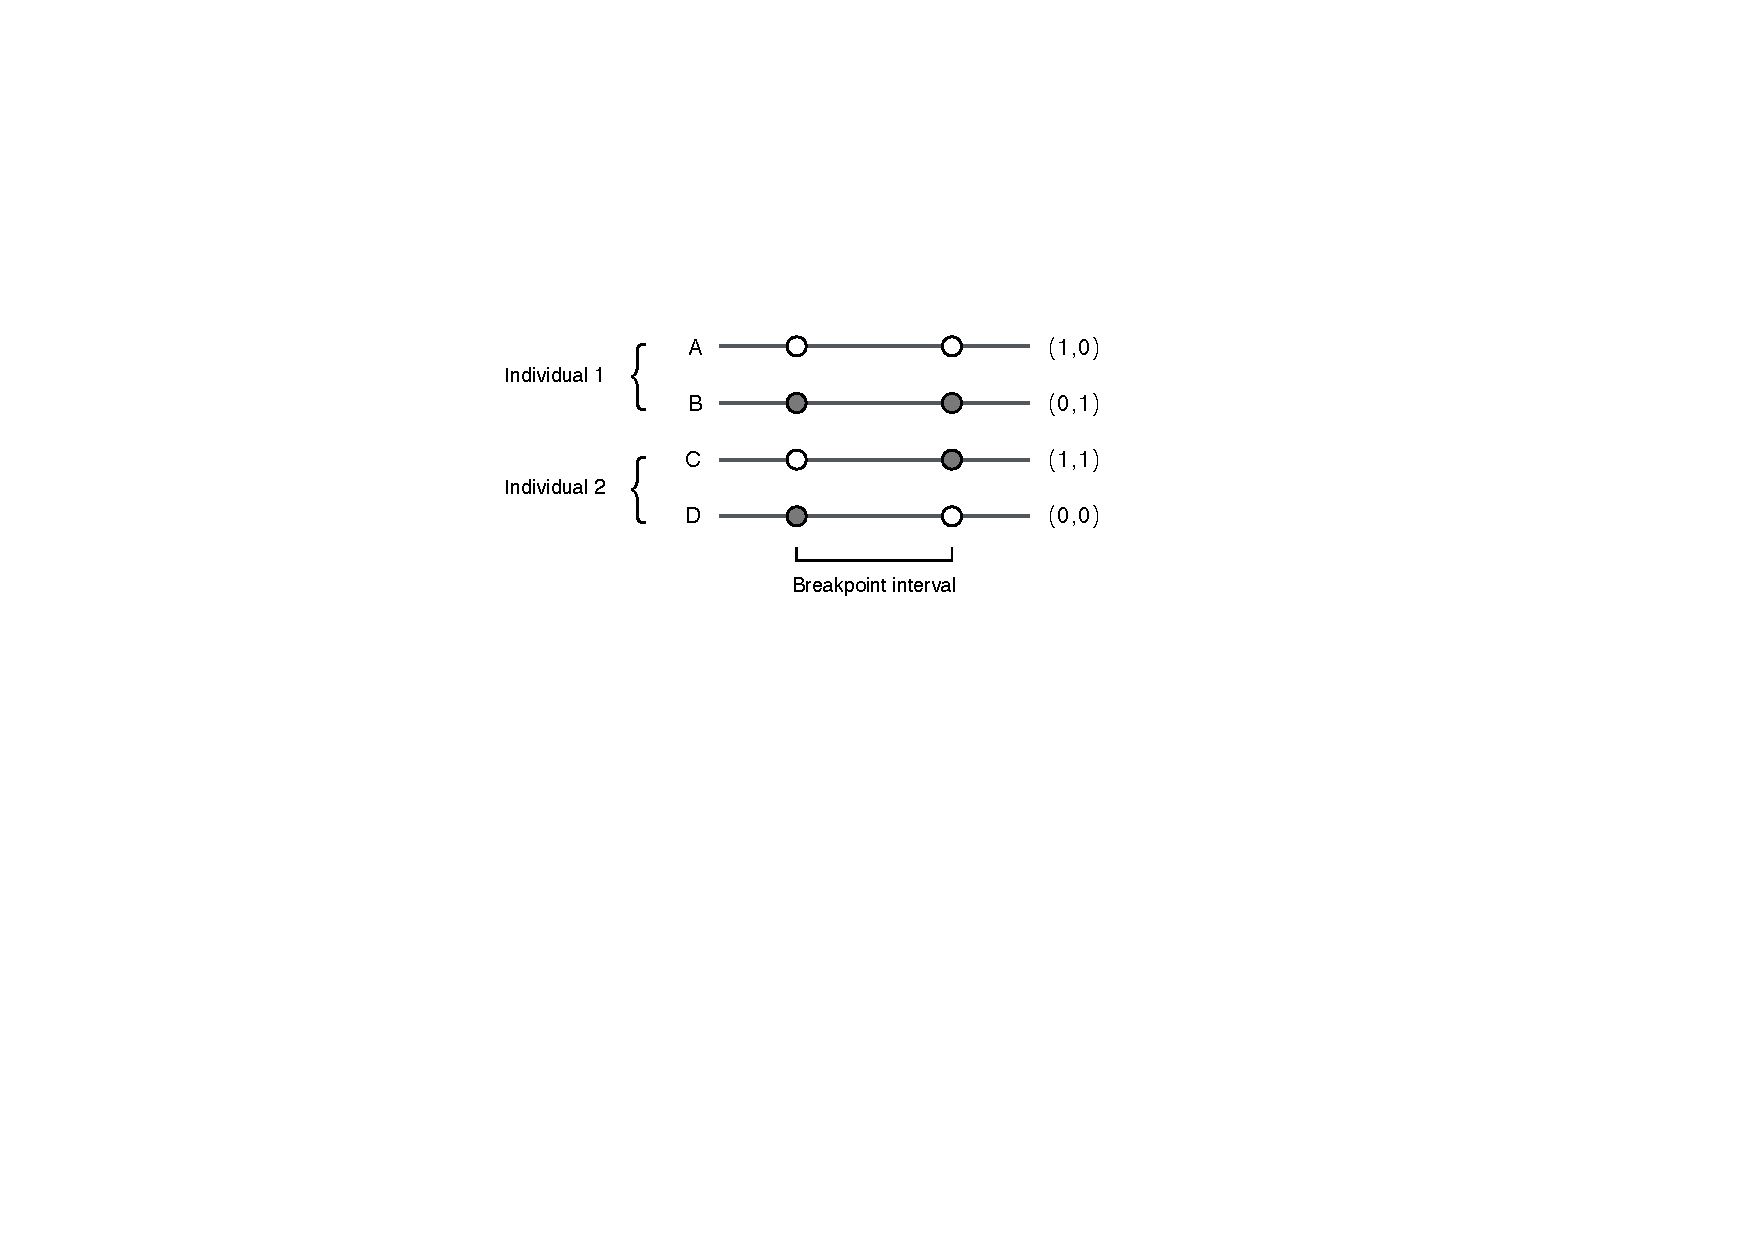
\includegraphics[width=0.7\textwidth]{./img/ch3/info_fgt}
\Caption{Breakpoint detection using the four-gamete test (FGT)}
{The \n{4} haplotypes (gametes) in a pair of \n{2} diploid individuals are shown (\emph{horizontal lines}).
A breakpoint interval is detected if all \n{4} possible allelic state configurations are observed at \n{2} variant sites along the sequence.
The interval delimits the region in which at least \n{1} recombination event must have occurred in the history of the sample (given the assumptions of the infinite sites model).
The \n{4} allelic state configurations are shown on the \emph{right}.
The alleles are shown at the \n{2} breakpoint sites; indicated as ancestral (\emph{hollow} circle) and derived state (\emph{solid}).
Note that the order of gametes is ignored.}
{fig:info_fgt}
\end{figure}
